
\section{\hspace*{3pt}  Topology Description}

A graph-theoretic analysis of the Wikipedia Category Graph was carried out to describe the topology of the graph and to estimate whether graph-based techniques for semantic analysis and information retrieval can be applied to the Wikipedia Category Graph.

The Wikipedia Category Graph assembled for the experiments contains $1,475,806$ vertices and $4,091,417$ edges. Each vertex represents a category and each edge represents a relationship of the type ``Subcategory Of". \textcolor{red}{[Sean: O que isto quer dizer? Isto é grande, pequeno, ruim, bom, comparado a que? Não são poucas aretas para o número de vértices (ou considerando hierarquia, seriam muitas?)?]}

If we observe a node in a directed graph, it is possible to see edges converging in the node and edges diverging from the node. An incoming edge and an outgoing edge can mean very different things, but in the Wikipedia Category Graph they both (I used this structure to reflect the fact that although they have different meanings, they have the same function in this case. A simple coordinating conjunction sounded vague.) denote the direction of the relationship ``is subcategory of". 

\subsection{\hspace*{3pt} Degree Analysis}

The indegree of node $v$ is the total number of connections onto node $v$, and is the sum of the $i$th row of the adjacency matrix: \textcolor{red}{[Sean: tem que explicar melhor a fórmula, descrevendo o que significa ``w", bem como ``a"]}
\begin{equation}
 k_v^{\text{in}}=\sum_w a_{vw}
\end{equation}

On the other side, the outdegree of node $v$ is the total number of connections coming (Do you mean "coming out"? Maybe "branch off"?) from node $v$ and is the sum of the $v$th column of the adjacency matrix:
\begin{equation}
k_v^{\text{out}}=\sum_w a_{wv}
\end{equation}

In both cases, the sum is over (I don't understand "the sum is over". Do you mean "The sum is the result of"?) all other nodes $j$ in the graph. It is also possible to sum indegrees and outdegrees to get the total number of connections of a node, which constitutes its total degree: 

 \begin{equation}
k_v^{\text{tot}} = k_v^{\text{in}} +  k_v^{\text{out}}
\end{equation}

The average indegree, outdegree and total degree for each vertex in the Wikipedia dataset are $2.78\pm0.142$, $2.78\pm0.001$ and $5.573\pm0.001$ respectively. \textcolor{red}{[Sean: o que isto representa?]}


\textcolor{red}{[Sean: faltou uma ligação entre os parágrafos]} The degree distribution of a graph is the probability distribution that a randomly chosen node will have a degree $k$. \textcolor{red}{[Sean: senti falta de uma explicação para que serve isto...]}

In directed graphs the degree distribution is a two-dimensional distribution, so that $P_{\text{deg}}(k^{\text{in}},k^{\text{out}} ) =$ the portion of nodes in the graph with indegree $k^{\text{in}}$ and outdegree $k^{\text{out}}$

Figure \ref{fig:in-and-out-degree} shows the degree distribution for the Wikipedia Category Graph in log space \textcolor{red}{[Sean: explicou log space? devo ter me perdido...]}. The $x$-axis shows the degree while the $y$-axis shows the count of nodes with such degree. \textcolor{red}{[Sean: senti falta de uma explicação mais detalhada da figura...]} 

\begin{figure}
\centering
\begin{subfigure}{0.49\textwidth}
\centering
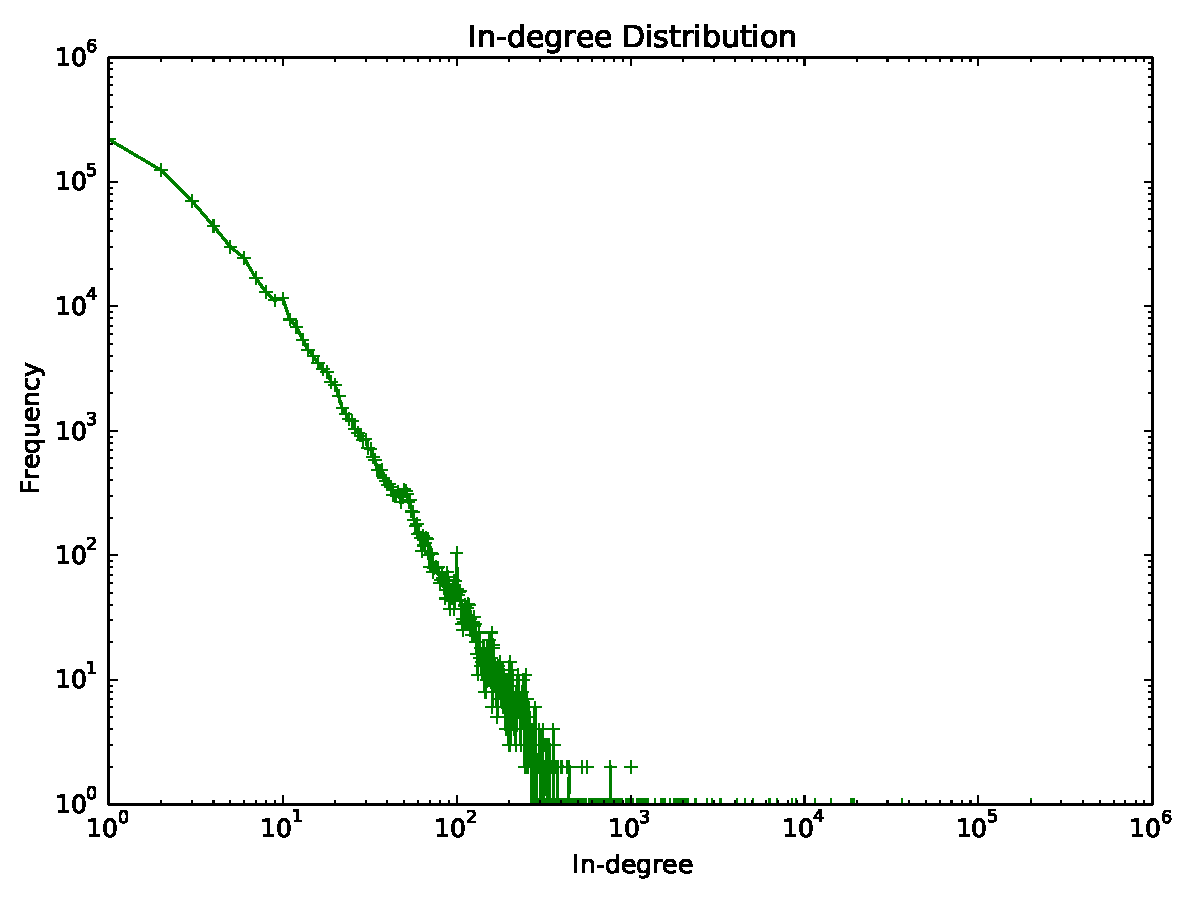
\includegraphics[width = \textwidth]{wikipedia-in-deg-dist.pdf}
\caption{Distribution of indegree}
\label{fig:left}
\end{subfigure}
\begin{subfigure}{0.49\textwidth}
\centering
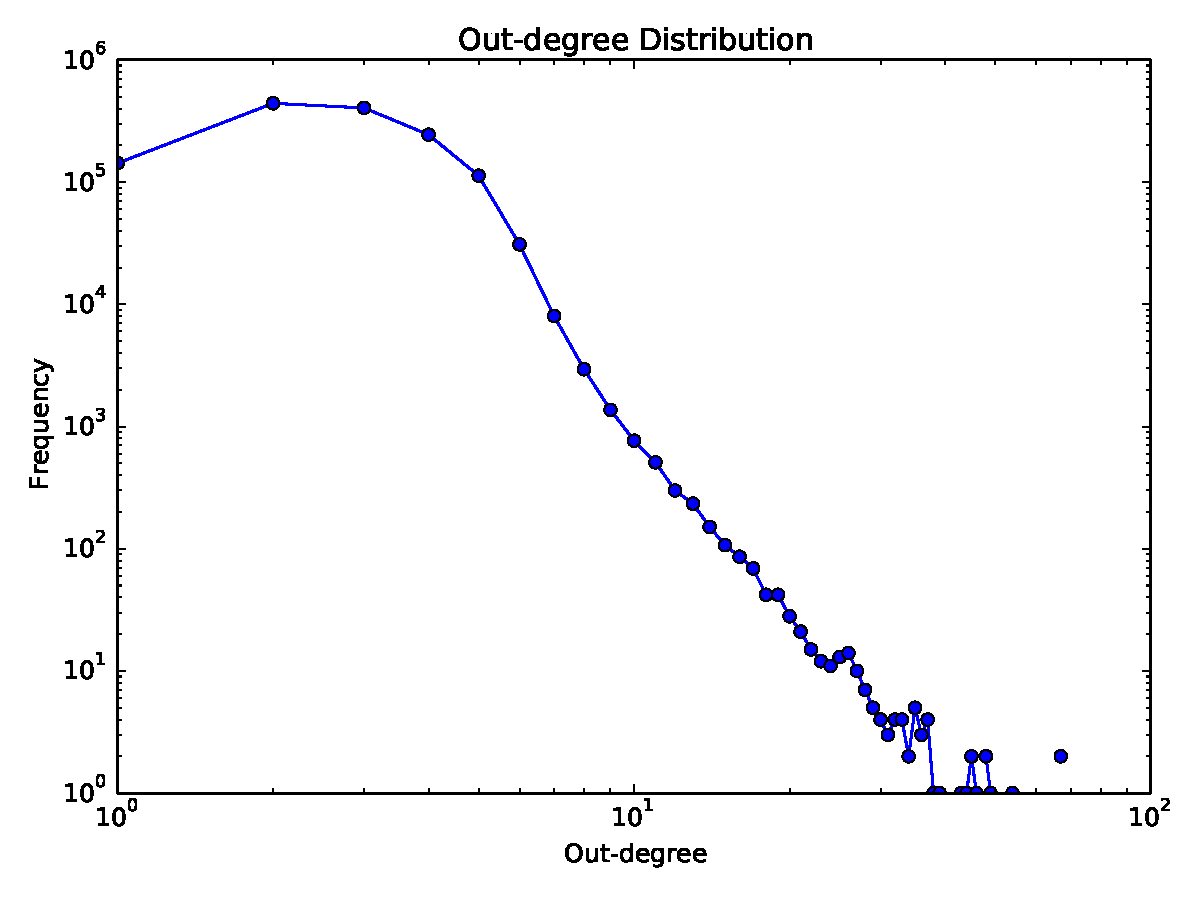
\includegraphics[width = \textwidth]{wikipedia-out-deg-dist.pdf}
\caption{Distribution of outdegree}
\label{fig:right}
\end{subfigure}
\caption{Indegree and outdegree distributions}
\label{fig:in-and-out-degree}
\end{figure}
Natural occurring networks tend to show a power-law \textcolor{red}{[Sean: explicar power-law]} distribution, which means that the fraction $P(k)$ of nodes in the graph having $k$ connections to other nodes varies as a power of some attribute $\alpha$, as in: 
\begin{equation}
P(k)=Ck^{-\alpha}
\end{equation}

This form of $P(k)$ decreases slowly as the degree $k$ increases, which multiplies the likelihood of finding nodes with a considerable degree.

A method for determining the coefficient of the power law is defined in \cite{clauset2009power} as \begin{equation}
\alpha = 1 +n\left[\sum_{i=1}^n\ln\frac{x_i}{x_{\min}}\right]^{-1}
\end{equation}
where $x_{\min}$ is a lower cutoff, below which the power law cannot be observed. 


\begin{table}[ht!]
\centering
\begin{tabular}{@{}lll@{}}
\toprule
           & $\alpha$ & $x\_{min}$ \\ \midrule
in-degree  & 2,4124 & 10         \\
out-degree & 4,5603 & 12         \\ \bottomrule
\end{tabular}
\caption{Power-law parameters of the Wikipedia Category Graph}
\label{tab:power-law-params}
\end{table}

Due to the fact that/Since power-law networks do not have a typical degree, they are referred to as scale invariants or scale-free networks, which are characterized by the presence of large hubs. \textcolor{red}{[Sean: então não entendi para que servem estes cálculos... me perdi de novo...]}

Regarding the degree distribution in a graph $G$, we can also determine the assortativity coefficient $r$, which measures how vertices of different types are preferentially connected amongst themselves. The assortativity coefficient \cite{newman2003mixing} is the Pearson correlation coefficient of degree between pairs of linked nodes. Positive values of $r$ indicate a correlation between nodes of similar degree, while negative values indicate relationships between nodes of different degree. In general, $r$ lies between -1 and 1. When $r = 1$, the network is said to have perfect assortative mixing patterns, when $r = 0$ the network is non\-assortative, and when  $r=-1$ the network is completely disassortative.

The assortativity coefficient $r$ is defined as
\begin{equation}
r = \frac{\sum_i e_{ii} - \sum_i a_i b_i}{1-\sum_i a_i b_i}
\end{equation} 
, where $a_i=\sum_je_{ij}$; $b_j=\sum_ie_{ij}$ and $b_j=\sum_ie_{ij}$ \textcolor{red}{[Sean: não entendi a repetição de bj = somatório]} is the fraction of edges from a vertex of type $i$ to a vertex of type $j$.  \textcolor{red}{[Sean: não entendi... senti falta de uma explicação mais textual sobre ``e", ``a" e ``b"]} The assortativity coefficient for our graph for indegree, outdegree and total degree are  respectively: 
$-0.0034$, $0.0898$, $0.0051$.  \textcolor{red}{[Sean: senti falta de uma explicação do que estes coeficientes querem dizer, quais as implicações...]}

Assortativity is high when high-degree nodes tend to connect to other high-degree nodes and it is low (i.e., negative) when high-degree nodes are linked to low-degree nodes. An assortativity of 0 indicates no correlation between the degrees of the nodes.


The density $D$ of $G$ is the ratio of edges in $G$ to the maximum possible number of edges, defined in a directed graph as  
\begin{equation}
D={\frac  {|E|}{|V|\,(|V|-1)}}
\end{equation}
\textcolor{red}{[Sean: Embora óbvio, talvez valha a pena explicar ``E" e ``V"]} A graph is said to be dense when the number of edges (shown?) is close to the number of possible edges. In the Wikipedia Category Graph the density is $1.878519 * 10^{-6}$. \textcolor{red}{[Sean: Explicar o que isto quer dizer, as implicações...]}

Another important metric for understanding the topology of a graph is its clustering coefficient. The clustering coefficient of a vertex represents the probability that if two of its neighbors are randomly chosen, they will also be connected by an edge. More precisely, if a vertex has $t$ neighbors, then there are $t(t-1)/2$ possible edges that connect those neighbors ("there are X edges that can possibly connect to those neighbours" What's possible here? The amount of edges or the connection to the neighbours?). The local clustering coefficient of a vertex is the fraction of the edges that actually appear in the graph (or 0 if the vertex has degree 0 or 1). Given the graph $G= (v,E)$ and a vertex $v \in V$, the clustering coefficient of $v$ is 

\begin{equation}\label{eq:cc1}
cc_1(v) = \dfrac{number of pairs of neighbors connected by edges}{number of pairs of neighbors}  
\end{equation} 

The clustering coefficient of a graph $G$ is the average of the local clustering coefficients $cc_1(v)$ of all vertices $v \in V$. The Wikipedia Category Graph has a clustering coefficient of $0.0461$. \textcolor{red}{[Sean: deveria explicar o que isto significa... discutir as implicações...]}

An alternative way of calculating the clustering coefficient of a graph, referred to as the global clustering coefficient or transitivity, was proposed by \cite{newman2001random}. \textcolor{red}{[Sean: Aqui a referência é ao autor, então deveria ser no formato autor [ref]]} Given the graph $G = (V,E)$ the global clustering coefficient of $G$ is
\begin{equation}\label{eq:cc2}
cc_2 = \dfrac{number of closed 2paths}{number of 2paths}
\end{equation}
A closed 2-path is a 2-path (A 2-path what?) where the end nodes are connected and form a triangle. For the Wikipedia Category Graph, the global clustering coefficient is $0.0036\pm0.005$. \textcolor{red}{[Sean: explicar o que isto significa e implicações...]}

The diameter $d$ of a graph $G$ is the maximum topological distance that can be found between two nodes in $G$. In order to find the diameter of a graph, the shortest path between each pair of vertices needs to be determined first. The greatest length of any of these paths is the diameter of the graph. Alternatively, we can define it as 
\begin{equation}
d=\max _{v\in V}\epsilon (v)
\end{equation}
It is worth noticing that the distance is determined based on the graph orientation (Distance is measured/determined? This is not clear.) \textcolor{red}{[Sean: não entendi... quis dizer sobre a direção do grafo (ou o grafo ser direcionado)?]}. In the Wikipedia Category Graph, the maximum topological distance is $52$ and the nodes with the longest shortest path are Bengali Culture and Politics of Bangladesh. \textcolor{red}{[Sean: faltou explicar o que representa esta distância topológica para a wikipedia... é muito ou pouco? em relação a que? Por que será que esta é a maior distância (do exemplo)?]}

A path in a graph is a sequence of alternating nodes and edges that starts with a node and ends with another node in such a way that adjacent nodes and edges in the sequence are incidental to each other \cite{newman2010networks}. Nodes or edges can appear in the same path multiple times, and the number of edges in a path is the length of that given path. If a graph is connected, then any node can be reached via a finite-length path starting from (branching off?) any other node. The shortest path between a pair of nodes is called a geodesic path and there can be more than one such path.

The average path length, a concept in the field of network topology, is defined as the average number of steps in the shortest paths (Did you mean "path" [singular]?) for all possible pairs of nodes in the graph. In directed graphs, the average path length is calculated as follows:

\begin{equation}
l_{G}={\frac  {1}{2 * n\cdot (n-1)}}\cdot \sum _{{i\neq j}}d(v_{i},v_{j})
\end{equation}

where $d(v_{1},v_{2})$ denotes the shortest distance between $v_1$ and $v_2$ and $n$ is the number of vertices in the graph $G$. 

If two nodes are disconnected (i.e. no path exists between them), the path length between these nodes is infinite. Consequently, if a graph contains disconnected components, the average shortest path length $l_G$ tends to infinity. In order to avoid it (What's "it"? Infinity?), it has been assumed that if $v_2$ \textcolor{red}{[Sean: aqui não seria $v_1$?]} can not be reached from $v_2$, $d(v_{1},v_{2}) = 0$ \textcolor{red}{[Sean: por que? se baseou em algum trabalho para fazer isto? se é infinito então não faria sentido assumir igual a zero...]}. As a result, the $l_G$ is considerable small ($0.05970$) and does not represent the real mean path length. For this reason, the shortest distance for all pairs of vertices in the graph was also calculated and the average path length is $20,9343$ \textcolor{red}{[Sean: Aqui só faz sentido se indicar alguma restrição como o cálculo ter considerado apenas aqueles pares de vértices que têm caminho entre eles... Ainda assim, acho que deveria justificar o fato de ter feito o cálculo assim, pois se o fato de não ter caminho é considerado infinito, então a soma é infinita... pra fazer diferente tem que ter justificativa...]}. The shortest path length distribution is displayed in figure \ref{fig:path-distribution}. \textcolor{red}{[Sean: teria que explicar os resultados da distribuição... Além disto, tem que explicar os eixos...]}

\textcolor{blue}{bpn: isso eh meio furada, pq eh small por 2 possiveis razoes:  1) tem muitos nós disconectados, ou 2) os caminhos são realmente curtos. }

\begin{figure}
  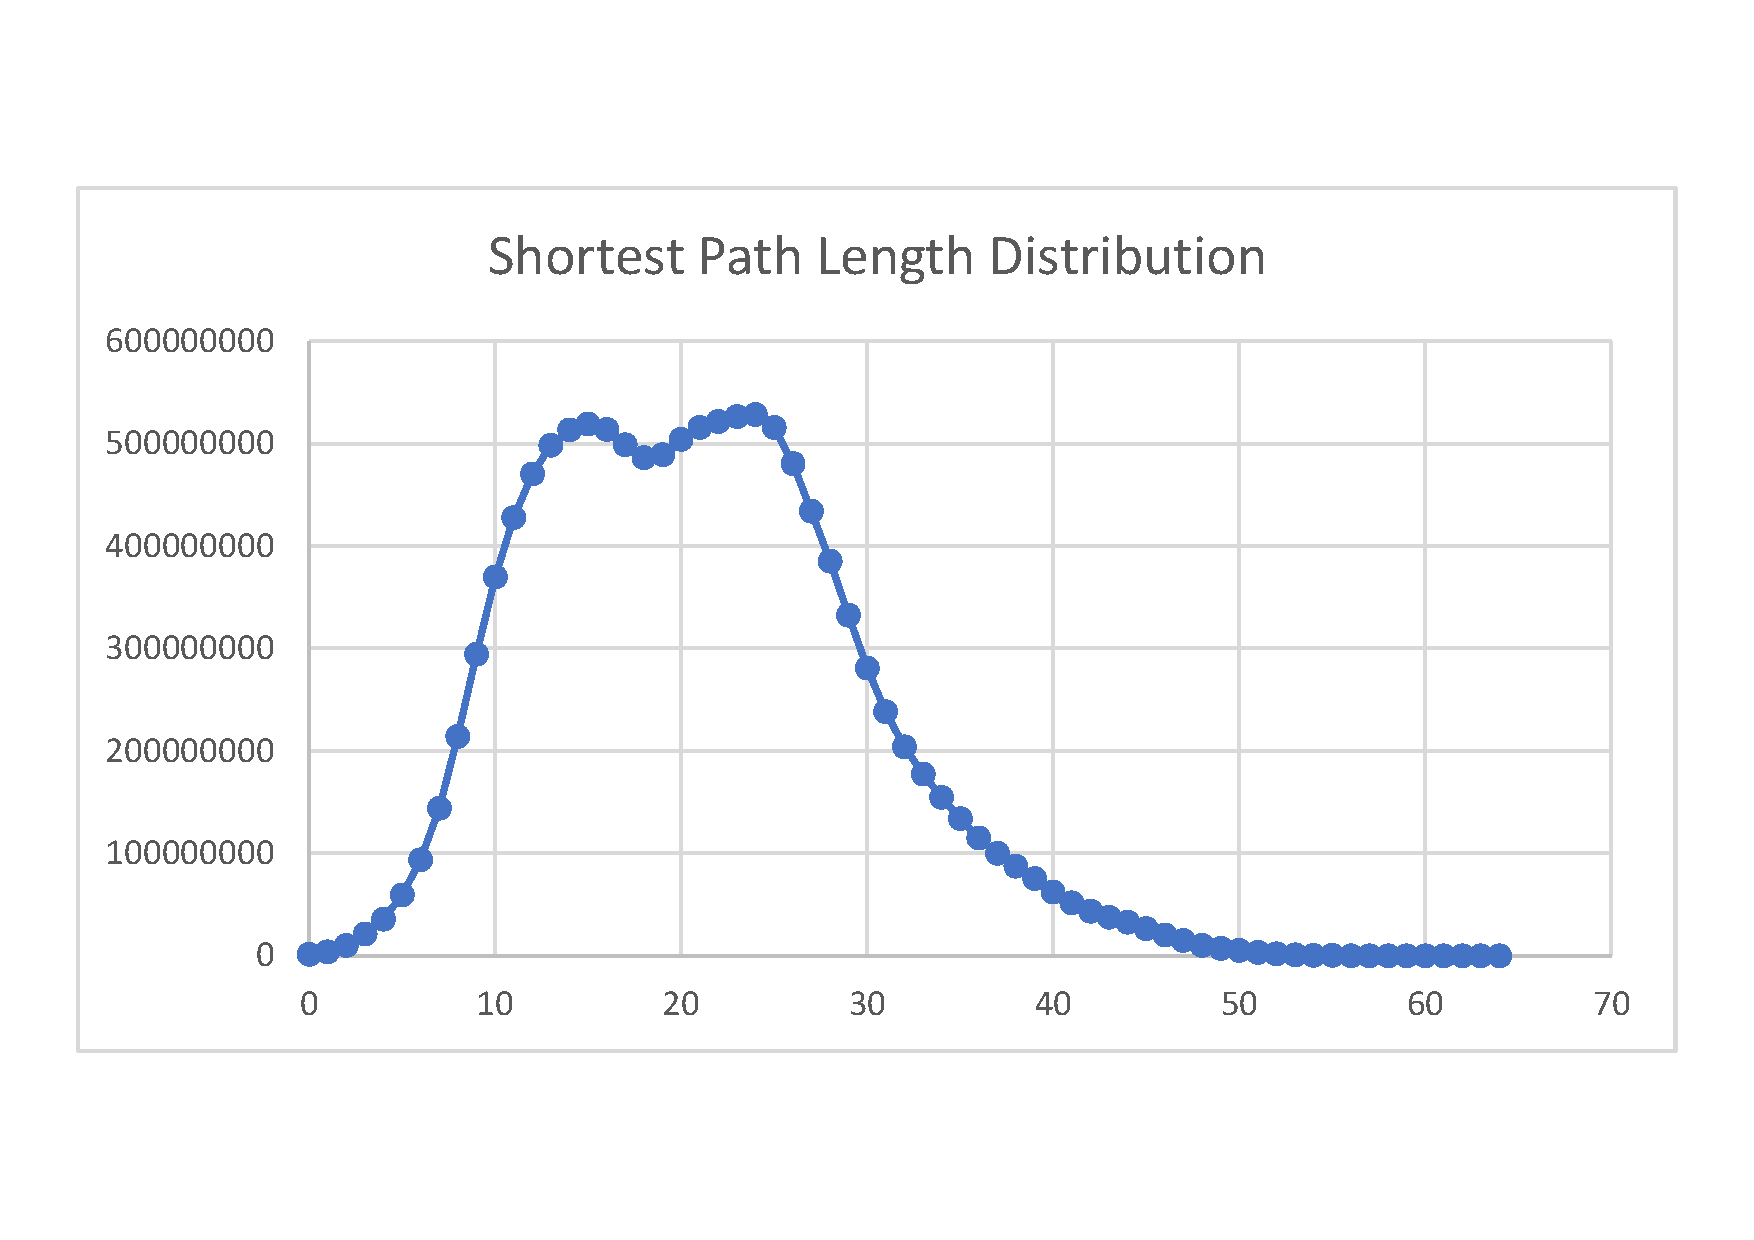
\includegraphics[width=\linewidth]{path_frequency2}
  \caption{Shortest path length distribution on th Wikipedia Category Graph}
  \label{fig:path-distribution}
\end{figure}

\subsection{\hspace*{3pt} Small World}
A small-world is a type of graph in which most nodes are not neighbors between them, but the neighbors of any given node are likely to be neighbors of each other, and most nodes can be reached from every other node by a small number steps (I got lost here.). Specifically, a small-world network is defined to be a network where the typical distance $L$ between two randomly chosen nodes grows proportionally to the logarithm of the number of nodes $N$ in the graph $G$ while the clustering coefficient is not small.

Formally, a graph $G$ with $n$ nodes and $m$ vertices is said to be a small-world if it has a similar path length but greater clustering of nodes than an equivalent Erdös-Rényi (E–R) random graph with the same $m$ and $n$. Let $L_g$ be the mean shortest path length of $G$ and $cc_{2_g}$ its clustering coefficient using the equation \ref{eq:cc2}. Let $L_{rand}$ and  $cc_{2_{rand}}$ be the corresponding quantities for the corresponding E–R random graph. According to the empirical experiments performed in \cite{watts1998collective}, a the (Not sure if "a" or "the" here.) graph $G$ is said to be a small-world network if
$L_g \ge L_{rand}$ and $ cc_{2_g} \gg cc_{2_{rand}}$.

In small-world graphs, the distance between any pair of nodes is relatively short while the level of transitivity, or clustering. is relatively high.

\textcolor{red}{[Crys: Eu acrescentaria um tópico de fechamento mostrando o que significa as coisas que você achou... por exemplo, o que significa seguir a lei de potência? Mas não tecnicamente... tipo... que indícios podem ter o fato de um grafo seguir a lei de potência. O que significa, o que representa, como eu interpreto um grafo small world.]}

\textcolor{red}{[Crys: Eu entendo que só o fato de extrair o grafo, aplicar as métricas e extrair as características do grafo já são contribuições importantes e VOCÊ PRECISA DIZER ISSO CLARAMENTE NA DISSERTAÇÃO. Então, mesmo que não consiga fazer o que coloquei no parágrafo anterior, você deveria fechar o capítulo dizendo o que me falou no áudio... que a extração dos dados, a construção do grafo e todas essas análises possuem um grau de dificuldade grande, devido à quantidade de dados. Explicar que até hoje poucos trabalhos fizeram isso, citar quais e as limitações. Argumentar que a construção e análise desse grafo traz a tona (feio isso, mas é mais ou menos nesse sentido) a estrutura das categorias de uma rica base de dados, blá blá blá... valorizar a importância de construção desse grafo. ]}




\begin{table}[!h]
\centering
\begin{tabular}{@{}lllll@{}}
\toprule
    & $L_g$       & $L_{rand}$       & $C_g$           & $C_{rand}$        \\ \midrule
WCG & 20,9343 & 19,5389 & 0,003638604 & 2,03E-06 \\ \bottomrule
\end{tabular}
\caption{Empirical demonstration of small-worldness of WCG \textcolor{red}{[Sean: não deveria ser $cc_{2_{rand}}$ ao invés de $C_{rand}$? E o mesmo para $cc_{2_{g}}$ e $C_{g}$]}}
\label{small-worldness}
\end{table}

Therefore, the Wikipedia Category Graph exhibits a small-world behavior, with an average shortest path length close to that of a random network with the same size.